\documentclass{article}%
\usepackage[T1]{fontenc}%
\usepackage[utf8]{inputenc}%
\usepackage{lmodern}%
\usepackage{textcomp}%
\usepackage{lastpage}%
\usepackage[head=40pt,margin=0.5in,bottom=0.6in]{geometry}%
\usepackage{graphicx}%
%
\title{\textbf{Avances tecnológicos impulsan la telemedicina}}%
\author{AFP}%
\date{04/03/2019}%
%
\begin{document}%
\normalsize%
\maketitle%
\textbf{URL: }%
http://www.eluniversal.com/estilo{-}de{-}vida/34336/avances{-}tecnologicos{-}impulsan{-}la{-}telemedicina\newline%
%
\textbf{Periodico: }%
EU, %
ID: %
34336, %
Seccion: %
estilo{-}de{-}vida\newline%
%
\textbf{Palabras Claves: }%
NO\_TIENE\newline%
%
\textbf{Derecho: }%
2.1%
, Otros Derechos: %
\newline%
%
\textbf{\textit{Gracias a estos grandes avances los doctores pueden desde la distancia evaluar y diagnosticar a los pacientes siendo más participativos aunque no estén presentes}}%
\newline%
\newline%
%
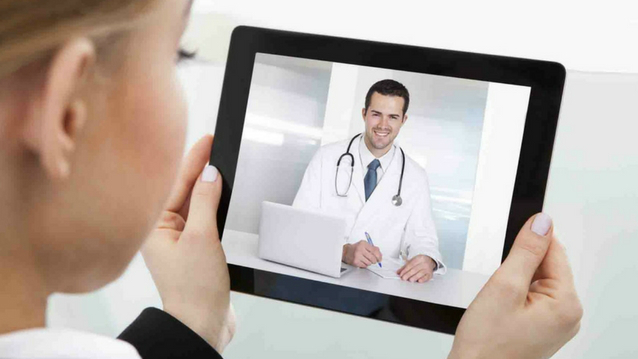
\includegraphics[width=300px]{EU_34336.jpg}%
\newline%
%
La telemedicina ha dado pasos agigantados, gracias a esto los doctores pueden vigilar la presión sanguínea, hacer pruebas auditivas e incluso participar en operaciones a distancia.%
\newline%
%
La tecnología móvil está sacando "la atención de salud fuera de las clínicas y hospitales", dijo Pamela Spence, especializada en ciencias de la salud en Ernst \& Young. \newline%
\newline%
Una muestra es la cabina de telemedicina desarrollada por la empresa francesa H4D que permite a un doctor a cientos de kilómetros de distancia medir el pulso, la temperatura o el nivel del oxígeno en la sangre de un paciente.%
\newline%
%
La cabina está equipada con herramientas que le permiten al médico hacer pruebas de audición y de visión, por ejemplo. \newline%
\newline%
Decenas de estas cabinas han sido instaladas en Francia, Italia y Portugal y la compañía está desarrollando programas piloto en Canadá, Estados Unidos, Filipinas y Dubái.%
\newline%
%
"Hace diez años la gente me veía como si fuera un extraterrestre", reconoció el fundador y presidente de H4D, Franck Baudino.%
\newline%
%
"La gente sigue pensando que somos de vanguardia, pero la gran diferencia es que hace diez años hablábamos del futuro, hoy son sistemas que están siendo usados", agregó este médico francés que trabajó en comunidades remotas en países en desarrollo. \newline%
\newline%
Para que el servicio tenga éxito, los médicos deben estar bien formados.%
\newline%
%
Lejos de la simple conexión telefónica entre médico y paciente, que quedó patente esta semana en el Congreso Mundial del Móvil (MWC), el mayor cónclave anual del sector celebrado en Barcelona. \newline%
\newline%
El gabinete de investigación de mercados Forrester predice que habrá más visitas virtuales al médico que en persona en Estados Unidos para finales de 2020.%
\newline%
%
"Hasta este momento, había habido un crecimiento lento en el mercado de la telemedicina", dijo Jeff Becker, experto en tecnología de cuidados de salud en Forrester. \newline%
\newline%
"Creemos que ya ha demostrado su utilidad en estos años y vamos a ver su adopción más amplia", insistió.%
\newline%
%
La llegada de las redes inalámbricas ultrarrápidas 5G, que empiezan a ser desplegadas por las operadoras de telecomunicaciones, abre nuevas posibilidades a la telemedicina, tales como cirugías realizadas a distancia controladas por robots.%
\newline%
%
Desde el MWC, el cirujano español Antonio de Lacy realizó la primera operación guiada a distancia usando la 5G. \newline%
\newline%
La red permitió a De Lacy una conexión en tiempo real con el quirófano del Hospital Clínic, a 5 kilómetros de distancia, donde un equipo médico intervenía a un paciente con un tumor intestinal.%
\newline%
%
"Es el primer paso para alcanzar nuestro sueño, que es hacer operaciones remotas en un futuro próximo", dijo. \newline%
\newline%
No es la primera operación guiada a distancia con redes inalámbricas, pero la 5G ofrece una calidad de imagen y una instantaneidad que reducen significativamente el riesgo de error.%
\newline%
%
La telemedicina puede ser especialmente importante en países en desarrollo con vastas áreas descubiertas por la red sanitaria. \newline%
\newline%
La aplicación Gifted Mom brinda a las mujeres en comunidades rurales alejadas en Camerún recomendaciones de salud de doctores de manera gratuita.%
\newline%
%
Para el 2020, espera haber reducido al menos un 70\% el número de mujeres que mueren al dar a luz en este país africano. \newline%
\newline%
Aunque muchos pacientes siguen prefiriendo un tratamiento en persona, el uso de la telemedicina "definitivamente" continuará, indicó Michael Barnett, profesor de la escuela de salud pública T.H. Chan de Harvard en Boston, que estudia las nuevas técnicas.%
\newline%
%
"La cuestión es saber donde se parará. Pero, por ahora, su uso sigue siendo poco común, por lo que tiene mucho espacio para crecer", afirmó.%
\newline%
%
\end{document}